%----------------------------------------------------------------------------   
\chapter{Mérések}
%---------------------------------------------------------------------------- 

A VoIP hívás monitorozására vonatkozó mutatók a hívásfolyam médiaútvonalának bármely 
csomópontján mérhetőek. Alapvetően számítással és összesítéssel történő elemzésre 
használják, és néha valós idejű teljesítménykövetésre és javításra is. \\

Ebben a fejezetben ismertetésre kerülnek a használt mutatók, tesztek menete és
azok eredményeinek összehasonlítása.

\section{Mutatók}

A következő mutatók kiszámolhatóak az RTCP csomagok alapján vagy maga az rtpengine
biztosítja számunkra a hívás végeztével.

\subsection{MOS és R-Faktor}

VoIP hívások minőségének mérésre két elterjedt mértékegység van az R-Faktor (osztályozási faktor)
és a MOS (Mean Opinion Score). MOS értéket gyakrabban lehet látni, viszont az R-Faktor szükséges
ahhoz, hogy kilehessen számolni a MOS-t. Az R-Faktor egy olyan mutató, ami a késleltetés, Jitter és
csomagvesztés mutatókból kerül kiszámításra. Az értéke egy 50-90 közötti szám, ahol 
az 50 rossz minőséget, míg a 90 kiválót jelent. 

A MOS a hang, videó és audiovizuális minőséget kifejező mértékegység az 
ITU-T P.800.1 szerint. A hallgatás, a beszéd vagy a párbeszéd minőségére utal, 
függetlenül attól, hogy szubjektív vagy objektív modellekből származnak-e. Ez a
mértékegység egy egytől ötig terjedő skálán mozog, ahol a legalacsonyabb a legrosszabb
és legmagasabb a legjobb minőség. Aminek a skálája a \ref{tab:mosValues} táblázatban 
lehet látni. 

\begin{table}[ht]
	\footnotesize
	\centering
	\begin{tabular}{l c c c c c c}
		\toprule
		 & Nagyon jó & Jó & Átlagos & Átlagtól rosszabb & Nagyon rossz & Nem ajánlott\\
		\midrule
		MOS & 5 - 4,3 & 4,3 - 4,0 & 4,0 - 3,6 & 3,6 - 3,1 & 3,1 - 2,6 & 2,6 - 1,0\\
		\bottomrule
	\end{tabular}
	\caption{MOS szintjei}
	\label{tab:mosValues}
\end{table}

%\begin{itemize}
%	\item Nagyon jó: 4,3 -5,
%	\item Rossz: 3,1 -3,6,
%	\item Nem ajánlott 2,6 - 3,1
%	\item Nagyon rossz: 1 - 2,6.
%\end{itemize}

%A \ref{eqMos} képletben lehet látni, a MOS kiszámítását, ahol az \textit{R} paraméter 
%az R-Faktor.
%
%\begin{equation} \label{eqMos}
%\text{MOS} = (((R-60) \cdot (100-R) \cdot 0,000007R) + 0,035R + 1)
%\end{equation}

A MOS rendelkezik alkategóriákkal is, ami a hívások különböző részeinek minőségét méri. A 
mérések során ebből csak kettő lesz felhasználva, a MOS-CQ (MOS Conversational Quality) és 
MOS-LQ (Listening quality). Az előbbi a társalgás minőségét míg az utóbbi a hallgatás minőségét
mutatja meg. \\

Azok a tényezők, amik befolyásolják a MOS és R-Faktor értéké a \ref{tab:values} táblázatban
vannak összefoglalva. 

\begin{table}[H]
	\footnotesize
	\centering
	\begin{tabular}{ l c c c}
		\toprule
		Mutató & Jó & Átlagos & Rossz\\
		\midrule
		Jitter & $\leq$ 10 ms & 10 ms - 30 ms & $\geq$ 30 ms\\
		Csomagvesztés & < 0.5 \%  & 0.5 \% – 0.9 \% & $\geq$ 0.9 \%\\
		Hangszint & > -40 dB & -80 dB - -40 dB & < -80 dB\\
		RTT & < 200 ms & 200 ms - 300 ms & > 300 ms\\
		\bottomrule
	\end{tabular}
	\caption{MOS számításnál használt mutatók jó és rossz tartománya.}
	\label{tab:values}
\end{table}


\subsection{Késleltetés}

Ez azaz idő, ami alatt a csomag egyik klienstől eljut a másikig ezredmásodpercben (ms). 

\subsection{Körülfordulási idő}

Az idő ami szükséges a csomagoknak, míg egyik klienstől eljut a másikig és vissza. SIP
hívások esetében ez azaz idő, amíg egy tranzakció tart, ami azt jelenti, hogy az elküldött
csomagra mennyi idő múlva érkezik egy nyugta. A szakdolgozat további részeben RTT (Round Trip Time)
fogja jelölni az angol neve után. 

Mérése ennek is ezredmásodpercben történik, mivel időről beszélünk, ezért minél magasabb ez a
szám annál rosszabb a hívás minősége. Az audiotartalom esetében a felső határ 150 ms, ami felett
már nagyon gyenge minőségű a hívás. Befolyásolhatja ezt a számot többek között, a kliensek 
közötti távolság, összeköttetés minősége és sávszélesség. A mérések során ezek mind nem fognak
változtatni az RTT idején, mert a szerverek "egymás mellett" vannak nagy sebességű kábelekkel
összekötve. Ami befolyásolni fogja, azaz a csomag útjában lévő proxyk mennyisége és azok feldolgozó
képessége. 

Fontos, hogy késleltetést nem lehet vele megbízhatóan mérni általános környezetben, mivel a hívó
felek között más útvonalak jelenhetnek meg, ami aszimmetrikus RTT eredményez. 

%Viszont az rtpengine ezt a számot nem adja meg konkrétan, szóval egy egyszerű számítást
%el kell rajta végezni, hogy a valós RTT-t megkapjuk.
%
%\begin{equation}
%\text{RTT} = \frac{\text{rtpegnine} \rightarrow \text{RTT}}{1000} + \text{rtpengine} \rightarrow \text{jitter} \cdot 2 + 10
%\label{calcrtt}
%\end{equation}

\subsection{Csomagvesztés}

Azon csomagok száma melyek nem jutottak el a céljukig. Szóval egyik klienstől a másikig. Ez különböző
indokok miatt történhet. A következő felsorolás nem teljes \cite{measure}

\begin{itemize}
	\item Nem elegendő sávszélesség. 
	\item Túlterhelés miatt nem képesek a felek feldolgozni a csomagokat.
	\item Tűzfalak, proxyk eldobják a csomagokat. 
\end{itemize}

\subsection{Jitter}

A kapott csomagok késleltetésének változása a folyam során. Méréséhez a csomagok küldési intervallumát
kell összehasonlítani a kapottak intervallumával. Szóval, ha két csomagot kiküldésre kerül 30 ms 
különbséggel és a kapott csomag 50 ms különbséggel érkezik, akkor a Jitter 20 ms. Ennél a mutatónál is
az előnyös, ha minél kisebb, mivel már egy kicsi Jitter és könnyen ronthat a hívás minőségén. 
Amik okozhatják:

\begin{itemize}
	\item A keret nagyobb, mint a Jitter puffer mérete. 
	\item Algoritmusok késleltethetik az interfészeken beérkező csomagokat. 
	\item A kommunikáció közben lévő hálózati eszközök, proxyk feldolgozó képessége. 
\end{itemize}

Javítani úgy lehet ezen a számon, ha az alkalmazások használnak Jitter puffert, ami elfogja a
beérkező csomagokat és azokat egyenletesen adja tovább feldolgozásra. 

\section{Tesztek menete és értékelése}

A tesztek oly módon történtek, hogy az általam írt kliens generált egy adott számú háttérforgalmat, 
majd a Linphone kliensekkel elindítottam egy rendest hívás, amivel könnyen lehetett a hívás minőségével
kapcsolatos információkat kapni. Ahhoz, hogy ez a rendszer megfelelően tudjon működni VirtualBox
segítségével egy hasonló környezetet teremtettem, mint a hagyományos hívásfelépítés részben.

Az így létrehozott Kamailio és két Linphone kliens egy-egy virtuális gépben futottak és ezek a gépek 
bridged hálózatot használtak, amelyek a \ref{fig:servers} ábrán látható Tethys enp12s0 és enp17s0
interfészekhez van hozzákötve. 

A tesztelés során elsőnek próbáltam minél nagyobb háttérforgalom mellett egy normál hívást elindítani,
viszont ez nem sikerült már 60-70 hívás esetén. Így ez lett a maximum szám kezelhető hívások száma. 
A probléma nem feltétlen a Kubernetes fürt túlterhelésében történt, hanem az L7mp proxyk kapacitásának 
elérése miatt. Így egy rendes Kamailio + Linphone által kezdeményezett hívást próbáltam indítani már 
nem volt képes a Kamailio ellenőrizni az rtpengine elérhetőségét egy \textit{ping} üzenettel, ezért
a klienseknek egymás elérhetőségét adta és szúrta be közéjük az rtpengine-t.

A diagramokon, táblázatokban szereplő adatok hálózati mérésekből lettek kinyerve. Ezeket a méréseket 
minden alkalommal az egyik Linphone kliensnél gyűjtöttem a \textit{tcpdump} nevezetű program. Ezzel 
a programmal csomagokat lehet elkapni és analizálni. Az így kigyűjtött csomagokat végül \textit{WireShark}
segítségével analizáltam. A WireShark lényegében ugyanazokat a funkciókat nyújtja, mint a tcpdump, azzal
a különbséggel, hogy a WireShark rendelkezik grafikus felülettel, ami könnyebb használni. 

\subsection{Mérések}

A legreprezentatívabb mutató a MOS, aminek a társalgási és hallgatósági minőségét lehet látni a \ref{fig:moslq}
ábrán.

\begin{figure}[!ht]
	\centering
	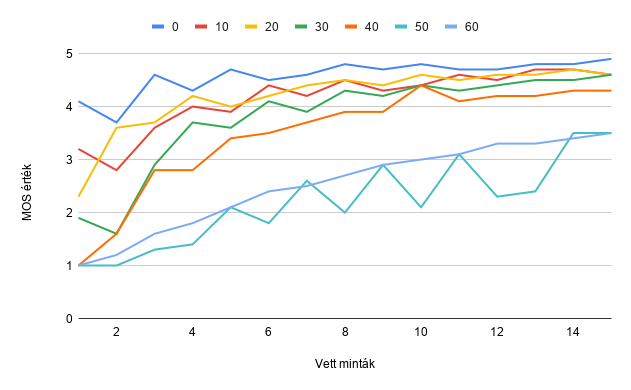
\includegraphics[width=1\textwidth, keepaspectratio]{figures/moslq.png}
	\caption{MOS-LQ változása az hívás során adott változó háttérforgalmak mellett.}
	\label{fig:moslq}
\end{figure}

Csak a MOS-LQ alakulása került ábrázolásra, mert a MOS-CQ-val szemben csak nagyon kevés különbség
van. Sajnos az ábrához nem tudtam jelmagyarázatot készíteni, így a vonalak színei jelképezik azt, hogy
mekkora háttérforgalom mellett voltak mérve a MOS értékek. Az Y tengelyen jelöli a vett mintákat, 
ami hívás kezdetétől számított és megvizsgált RTCP csomagokat jelöli. Mivel nem sikerült minden hívást 
egyforma hosszúságúra hagyni és tekintettel arra, hogy nagyobb terhelés mellett az első pár ilyen 
RTCP csomagban nem értelmezhető adatok voltak. Így az első 15 értelmezhető mintát vettem. \\

%\begin{figure}[!ht]
%	\centering
%	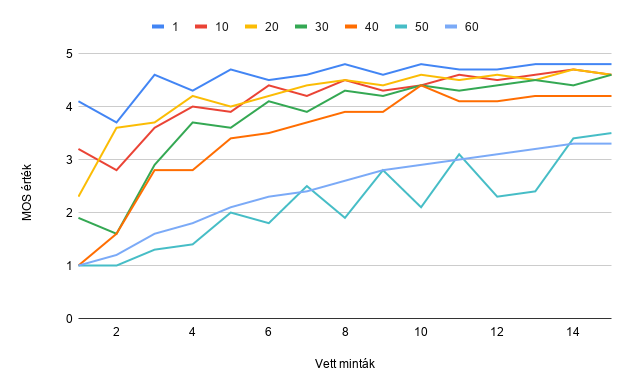
\includegraphics[width=1\textwidth, keepaspectratio]{figures/moscq.png}
%	\caption{MOS-LQ változása az hívás során adott változó háttérforgalmak mellett.}
%	\label{fig:moscq}
%\end{figure}

A \ref{fig:moslq} ábrán jól látható az folyamat, hogy a hívás kezdte után mennyire rossz a hívás minősége
illetve, hogy egy idő után mennyire javul és vesz fel egy viszonylag kis kilengésekkel rendelkező értéket. 
A hívás elején tapasztalható rossz minőséget az okozza, hogy az okozza, hogy az L7mp proxyk nem képesek
elég gyorsan feldolgozni a csomagokat így a magas Jitter keletkezik a rendszerben, amikre nincs
felkészülve egyik Linphone kliens sem. Később azért lesz jobb a MOS értéke, mert a kliensek adaptív
Jitter pufferel rendelkezni így idővel megtanulják azt, hogy mekkora az átlagos Jitter és annak megfelelően 
növelik a pufferük méretét. Így a magas Jitter értéket kitudja simítani.

De ez nem jelenti azt, hogy a hívás maradéktalanul jó lesz, amit mutat a következő \ref{fig:voiceComp}
ábra is, amit a WireShark RTP folyam elemzőjéből mentettem ki. 

\begin{figure}[!ht]
	\centering
	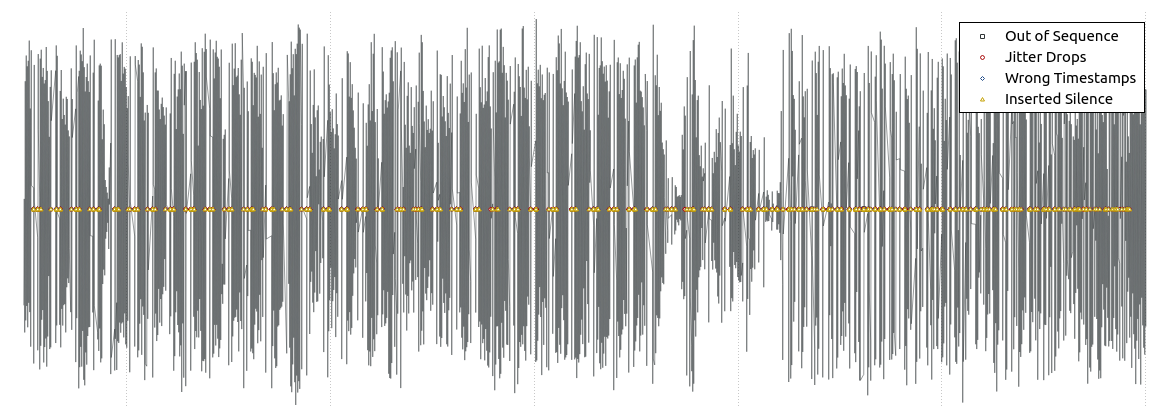
\includegraphics[width=1\textwidth, keepaspectratio]{figures/calls60.png}
	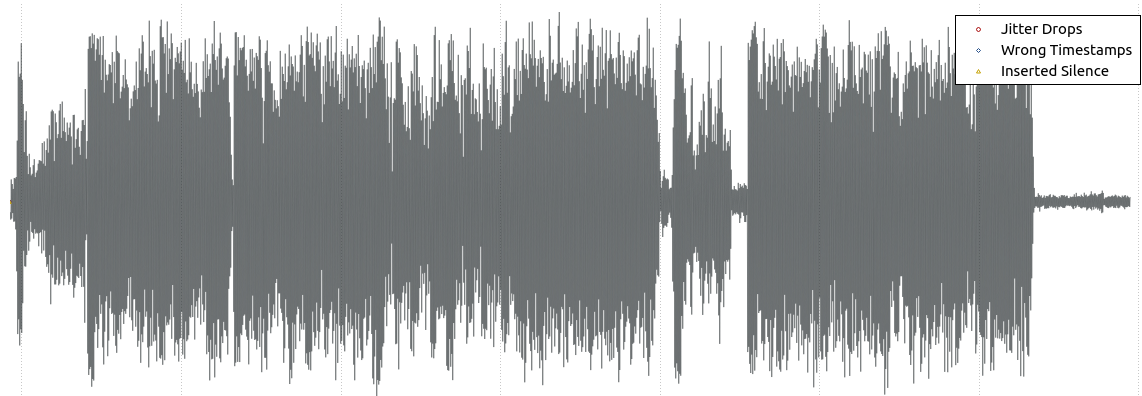
\includegraphics[width=1\textwidth, keepaspectratio]{figures/calls20.png}
	\caption{MOS-LQ változása az hívás során adott változó háttérforgalmak mellett.}
	\label{fig:voiceComp}
\end{figure}

A \ref{fig:voiceComp} ábrán a felső hullám 60 hívás mellett készült, míg az alsó 20 hívás mellett keletkezett. 
Ezek azok a RTP folyamok, amik az rtpengine felől érkeztek a kliensek felé. 

Jól látszik, hogy a felsőnél rengeteg csend van beszúrva, ami nagyon recsegőssé teszi a hívást és élvezhetetlenné,
míg az alsónál csak az elején található egyszer egy magas Jitter érték, ami nem befolyásolja annyira a hívás
minőségét. \\

\begin{table}[H]
	\footnotesize
	\centering
	\begin{tabular}{l c c c c c c c}
		\toprule
		 & 0 & 10 & 20 & 30 & 40 & 50 & 60\\
		\midrule
		MOS-LQ & 4,7 & 4,4 & 4,5 & 4,2 & 3,9 & 2,8 & 3,1\\
		MOS-CQ & 4,7 & 4,4 & 4,5 & 4,2 & 3,9 & 2,8 & 2,9\\
		R-Faktor & 94 & 88 & 90 & 84 & 78 & 55 & 59\\
		RTT & 17 ms & 9 ms & 17 ms & 16 ms & 16 ms & 42 ms & 182 ms\\
		Jelszint & -3 & -2 & -4 & -3 & -2 & -8 & -2\\
		Zajszint & -11 & -11 & -12 & -13 & -10 & -22 & -10\\
		Jitter & 2 ms & 7 ms & 13 ms & 5 ms & 66 ms & 69 ms & 173 ms\\
		Max Jitter puffer & 104 ms & 41 ms & 75 ms & 64 ms & 75 ms & 89 ms & 234 ms\\
		\bottomrule
	\end{tabular}
	\caption{Adott háttérhívás mellett mért mutatók átlagai.}
	\label{tab:callValues}
\end{table}

A \ref{tab:callValues} táblázatban jól látszik, hogy a hívások minősége miként romlott annak függvényében, hogy
hány háttérhívás volt egyszerre. Ami rögtön észrevehetőm, hogy a MOS értéke az folyamatosan rosszabb attól függetlenül,
hogy a \ref{fig:moslq} ábrán az látható, hogy idővel javul ennek az értéke. Ez attól van, hogy itt már az összes 
értelmezhető RTCP üzenet fel lett dolgozva és egy idő után beállt a MOS értéke egy adott szintre, ezért folyamatos 
csökkenés látható. 

A másik ilyen könnyen jellemezhető érték azaz R-Faktor, ahol jól látszik, hogy nulla háttérhívás mellett átlagosan 
sikerült elérni azt a minőséget, ami majdnem tökéletesnek számít. Ezt a viszonylag jó értéket tartja egészen 
40 hívásig, ahol is már egy nagy esés látható. Ez már azt jelenti, hogy élvezhetetlen a hívás. Ennek kiváltó 
oka lehet a magas Jitter, ami már ennyivel képes torzítani a hívást. A Jitter egész elviselhető értékeket adott 
40 hívásig, viszont azután már túl nagyok voltak, mivel 60 ms alatt nagyjából három RTP csomagnak kellett volna érkeznie.

A Linphone 60 ms-s Jitter pufferrel rendelkezik alap esetben és, ha szükség van rá, akkor ezt képes módosítani. Ez
látszik a táblázat utolsó sorában is, mivel adaptívan növeli puffer méretet. 